\documentclass{sigchi}

% Use this command to override the default ACM copyright statement (e.g. for preprints). 
% Consult the conference website for the camera-ready copyright statement.

%% EXAMPLE BEGIN -- HOW TO OVERRIDE THE DEFAULT COPYRIGHT STRIP -- (July 22, 2013 - Paul Baumann)
% \toappear{Permission to make digital or hard copies of all or part of this work for personal or classroom use is 	granted without fee provided that copies are not made or distributed for profit or commercial advantage and that copies bear this notice and the full citation on the first page. Copyrights for components of this work owned by others than ACM must be honored. Abstracting with credit is permitted. To copy otherwise, or republish, to post on servers or to redistribute to lists, requires prior specific permission and/or a fee. Request permissions from permissions@acm.org. \\
% {\emph{CHI'14}}, April 26--May 1, 2014, Toronto, Canada. \\
% Copyright \copyright~2014 ACM ISBN/14/04...\$15.00. \\
% DOI string from ACM form confirmation}
%% EXAMPLE END -- HOW TO OVERRIDE THE DEFAULT COPYRIGHT STRIP -- (July 22, 2013 - Paul Baumann)


% Arabic page numbers for submission. 
% Remove this line to eliminate page numbers for the camera ready copy
\pagenumbering{arabic}


% Load basic packages
\usepackage{balance}  % to better equalize the last page
\usepackage{graphics} % for EPS, load graphicx instead
\usepackage{times}    % comment if you want LaTeX's default font
\usepackage{url}      % llt: nicely formatted URLs
\usepackage{enumerate}
\usepackage{mathtools}
\usepackage{color}
\usepackage[round]{apalike} % to use APA style bibliography



% llt: Define a global style for URLs, rather that the default one
\makeatletter
\def\url@leostyle{%
  \@ifundefined{selectfont}{\def\UrlFont{\sf}}{\def\UrlFont{\small\bf\ttfamily}}}
\makeatother
\urlstyle{leo}


% To make various LaTeX processors do the right thing with page size.
\def\pprw{8.5in}
\def\pprh{11in}
\special{papersize=\pprw,\pprh}
\setlength{\paperwidth}{\pprw}
\setlength{\paperheight}{\pprh}
\setlength{\pdfpagewidth}{\pprw}
\setlength{\pdfpageheight}{\pprh}

% Make sure hyperref comes last of your loaded packages, 
% to give it a fighting chance of not being over-written, 
% since its job is to redefine many LaTeX commands.
\usepackage[pdftex]{hyperref}
\hypersetup{
pdftitle={SIGCHI Conference Proceedings Format},
pdfauthor={LaTeX},
pdfkeywords={SIGCHI, proceedings, archival format},
bookmarksnumbered,
pdfstartview={FitH},
colorlinks,
citecolor=black,
filecolor=black,
linkcolor=black,
urlcolor=black,
breaklinks=true,
}

% create a shortcut to typeset table headings
\newcommand\tabhead[1]{\small\textbf{#1}}


% End of preamble. Here it comes the document.
\begin{document}

\title{Improved usability in distributed interactive system for collaborative affinity diagram: an experimental  comparison of digital vs. analog}

%\numberofauthors{1}
%\author{
 % \alignauthor William Widjaja\\
 %   \affaddr{Department of Management of Science and technology, Tohoku University}\\
 %   \affaddr{Aobayama 6-6-01-2, Sendai, Japan}\\
  %  \email{william.widjaja@most.tohoku.ac.jp}\\
 }
\maketitle
\begin{abstract}
Affinity diagrams are a popular method for creating and organizing ideas. While there are many digital solutions for affinity diagram creation, they have not been widely adopted due to usability challenges, so teams still use the analog method more often. Distributed Affinity Diagram System (DADS) is a system that aims to solve the existing usability problems with this type of groupware and present a more usable solution than the analog method. DADS proposes a dual-screen terminal that divides private input space from common interactive space in each user's setup. While private input encourages users to create and nurture ideas, common interactive spaces are designed to sync all users' actions across all terminals, allowing users to collaborate interactively through a distributed multi-touch system. The separation of input space and the distributed synchronized interactive space can improve usability, efficiency, and user satisfaction. We present experimental evidence comparing DADS to the traditional analog method of collaborative affinity diagram creation in order to prove our claims.

\keywords{
	CSCW;Collaboration; Affinity-Diagram; Brainstorming; Group work; Sticky-note ; Groupware
}

\section{Introduction}

Group problem solving involves exchanging and organizing ideas in order to come up with a satisfactory solution. Affinity diagrams, also known as the KJ method, are a popular discussion organizing tool\cite{kawakita1991original}. Affinity Diagrams are often created by writing individual points on sticky notes or cards and, together with other participants, sorting the cards to uncover the points' similarities. Collaborative affinity diagrams can be useful tools for problem solving because they give discussions structure and explicit goals. This gives groups a tried and tested method to generate and refine ideas in search of the best. 

Three important parts of the collaborative affinity diagram determine its quality: Input, Presentation, and Collaboration. Input can be pen and paper, digitally captured writing, typed text, drawings, or any other media. Users want to contribute their ideas to discussion easily, using familiar tools. Usable collaborative systems will give users a familiar setting and make inputs easy to create. Presentation creates greater understanding between all team members, which means that a high-quality system must let users present and explain their ideas to each other easily. Collaboration requires flexibility in the tools available for communication. Collaboration will be more efficient if users are able to communicate their thoughts in different formats and be uniquely identified as the source of their ideas.

While most uses of the affinity diagram employ sticky notes to represent individual points, the method does not require physical objects to represent users' ideas, and several digital implementations of the collaborative affinity diagram method have been developed, including our own. Indeed, the recent trend toward a paperless office means that paperless implementations of collaborative tools deserve further research. However, the most common implementation of digital collaborative affinity diagrams is to create a monolithic single group display. There is a long tradition of computer supported collaborative work that we can build on to encourage interaction through technology while protecting an individual idea-space. Below, we discuss the state of the art systems with innovations in input, presentation, and collaboration. These systems have inspired us to search for a solution to challenges in groupware for brainstorming and discussion. 

Pen and paper are flexible tools for creation and collaboration, and many teams prefer to use analog methods over groupware for discussion. Designers and researchers have taken note of this preference and created systems that allow users to keep their analog tools. Input from analog methods can be digitized using a variety of technology. Some systems digitize user input with image-capturing software and a video camera that captures the collaborative space. Earlier researchers  used an overhead camera to capture users' drawings and writing below the tabletop interactive spaces\cite{klemmer2001designers, steimle2009coscribe,hartmann2010pictionaire}. Other designers have built systems around the Anoto digital pen which uses microdot printed paper to track the pen location and convert the analog writing input into digital text \cite{haller2010nice,miura2011gkj, ispas2010paper, Geyer:2011:DRI:2069618.2069647}. Some systems allow users to create an input using a distributed interface such as PDA, mobile phone, or tablet \cite{ballendat2010proxemic,greenberg1999pdas,burtner2013affinity,Geyer:2011:DRI:2069618.2069647}. These systems give users a personal space to nurture ideas without interruption by other activities. However, many of these distributed systems are still focused on a monolithic shared group display (SGD) and specialized technology, such as an overhead projector and camera, or digital pen and microdot paper  as in the Anoto pen system. We think it is important to give users a familiar setup to express their thoughts. Access to a familiar system with a keyboard, mouse, and browser will allow users to efficiently research, build and nurture ideas. It is important for ideas in discussion to be well developed in order to be understood by everyone, many available affinity diagrams are designed to generate simple written ideas or opinions without in depth description or supporting documents.  So far, current groupware research has not focused on systems that increase users' understanding by providing more depth of information on discussion points.

%Another important factor is the ability in share and present ideas with others, most of the system done a very good job by presenting ideas and large images such as photos table graph , smaller text based sources  from the internet website are not easy to present which allow users to only show big pictures. It is also important for users to be able to control the presentation each by themselves, . While huang and judge pointed out the problem using a single group display for real case discussion, due the interaction overload and difficulty in explaining their points to others people, so far we think that in depth presentation such as well organized  discussion points and curated sources are still not being prioritize by other researchers to increase the ease of presentation and context understanding of the discussion topics. 


Single Group Displays (SGD) seem to be the preferred method of collaboration for increased gaze awareness and large visual bandwidth for collaboration. Issues with using SGDs in real cases are explored in research by Huang et al., who suggest that single group displays proved to have serious problems with interaction and social overhead in the real world scenario. Judge et al. \cite{judgeusing} also suggest that a challenge for SGD users is that they are unable to identify their own points. This lack of point identification stems from two things: the ideas represented by the point card are rarely tied to the author of the card, and SGDs lack a way to differentiate which touches on the screen belong to which users. While it is easy to solve the first problem of identifying sticky notes through better software design, it is harder for single group displays to track users and link them to their ideas. Despite this, Ramakers et al \cite{ramakers2012carpus} adapted an overhead camera system to identify users' hands during collaboration, and Tang \cite{tang2004videoarms} uses the same method to add a shadow arm indicating the presence of a user during discussion. Haller's Nice discussion \cite{haller2010nice} solution uses a specialized digital Anoto pen which detects two different users. This allows users to digitally collaborate with each other using different colored pens, just as they would in the analog method. While these solutions solve the problem of identification, the monolithic aspect of SGD technology may still impact usability. Gumienny and colleagues' work on Teleboard \cite{gumienny2011tele} uses a new approach of distributed whiteboard system for long distance collaboration. We think this is a promising start that solves some of the issues with SGD systems, but further integration with meaningful input is needed to ensure that this technology will mature into a usable and efficient solution. Despite the potential of these systems, very few digital affinity diagram systems have been widely adopted in real-world scenarios.


\section{Hypotheses and Proposed Solutions}
\begin{figure}[!h]
\centering
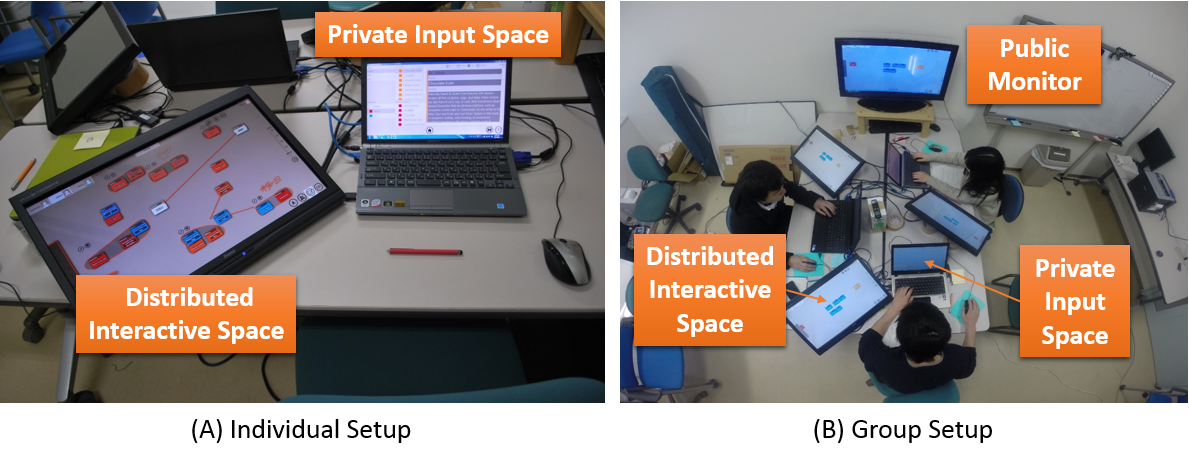
\includegraphics[width=1.0\columnwidth]{indigro}
\caption{(A) Single Individual Setup with Dual monitor(B) Group Setup with U-shape seating with a main monitor at the end of the table}
\label{fig:figure1}
\end{figure}

The above challenges have prevented people from switching to digital tools despite the potential benefits. This paper aims to provide a system with better usability compared to analog methods. The system we have developed to solve these challenges is called the Distributed Affinity Diagram System(DADS). It is an individual terminal setup with a dual monitor system. The main screen is used for web research and input of ideas and points, and an extended multi-touch screen is used for interactive collaboration. In addition, we created an algorithm that synchronizes all users' actions in the collaborative space across all terminals. This algorithm is designed to be highly responsive and allow users to naturally control the movement of assets in the interactive space. Smart algorithms were also designed to give each user an identity. Clash prevention and resolution measures are integrated in the system to ensure that the system is resilient to users' simultaneous and varied actions. This solves many of the challenges faced by current digital affinity diagram systems in the field of CSCW research. 
We believe that this system can give users increased usability and efficiency of collaboration beyond what is available using the analog method. We aim to address four specific areas in which the usability of digital affinity diagram creative activities can be improved. These four areas are: (1) increasing the efficiency of content creation, editing and navigation, (2) improving capacity for information source attachment, (3) making presentation to others easier, (4) and increasing flexibility in collaborating on the affinity diagram. Upon completing these improvements, we conducted a user test to determine whether the system's usability was improved. 
\begin{figure*}
\centering
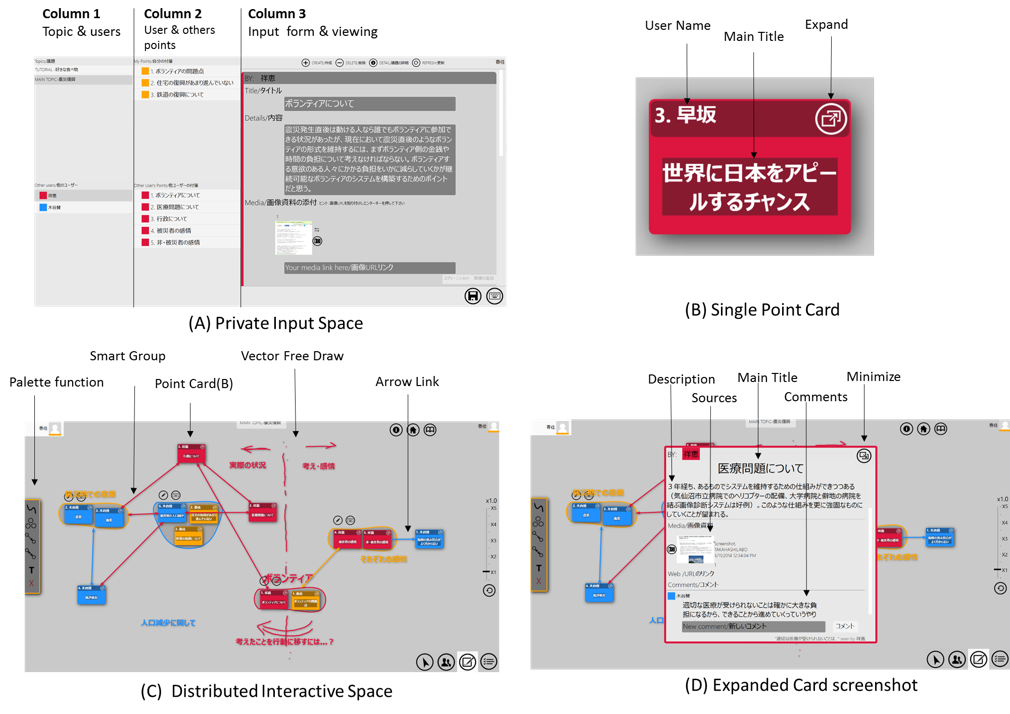
\includegraphics[width=1.7\columnwidth]{all}
\caption{A) Private Input Interface B) Individual Points  C) Distributed Screen  D) Expanded Card Interface }
\label{fig:figure1}
\end{figure*}

\subsection{(1) Efficient Content Creation and Editing} We hypothesize that keyboard-based digital input  can make content creation and editing easier in the context of collaborative affinity diagrams, as long as users can access the affinity diagram without negotiating for personal space with other users. In traditional affinity diagram creation, we observed that users spent time waiting for others to post and move cards. This time could be better spent creating points or thinking about how to arrange points in meaningful groups. For this reason, we designed our system to provide a dual screen interface, where one screen is dedicated to creating and organizing one's own points. We also hypothesize that good user interface design can improve navigation and increase information flow between users' discussion points, leading to improved understanding of other users' points. Our system provides an intuitive 3-column interface (shown in Figure 1(A)) in which users create new items and populate them with content, and easily switch back and forth between viewing their own and others' points. The point viewing section is divided into two areas (Title and Contents) which can help users formulate their points more clearly. Users can toggle between their own and others' points quickly and without using a menu, which will improve the efficiency of navigation. Users are identified by a unique color associated with their points both in the private interface and on the common board. %It was important to us in designing the system that we retain familiar design features that make users comfortable with input methods, while also making improvements that enable users to collaborate with each other smoothly and efficiently. 
\subsection{(2) Attaching Internet Sources} No current research focuses on the effective use of external sources in computer-mediated discussions. We hypothesize that sources would help users to better explain their points to others, and also make it easier for them to understand others' points. The attachment system that we have designed for DADS allows users to support their points using multimedia sources by cutting and pasting, selecting images, or capturing a screen shot of any website. %URLs and images are processed into a thumbnail format that can be expanded by the user or viewer.  In analog affinity diagram creation, people would be able to easily print materials and paste them on the board next to their point; however, a system that integrates source attachment functions will more efficiently promote the use and understanding of sources that support users' points.
\subsection{(3) Presenting Points and Sources} Part of our integrated system is a presentation tool that can be used to make points easier to explain and easier to understand. Our proposed solution capitalizes on users' separate screens: since each user has her own screen, presentation can take place on a distributed synchronized screen in which discussion points are in card format, with only their title displayed. Details for each point can be expanded on all users' screens (as in Figure 2(D)) synchronously, under the control of one user at a time, so that each user can present their own ideas points. %When the system is in presentation mode, card and image expansions are synchronized across all users' common interactive boards and the central common view screen. In addition, a special digital pointer tool lets users highlight areas of the screen or indicate a certain passage of text. 
%\subsection{(4) Organizing Comment Exchanges } While speaking would be an easier and faster way to exchange comments, one drawback of speech is that it is hard to maintain a record of what was said. Since discussions involve multiple points, collaborative discussions can benefit from a method for coordinating which point should be discussed next. text-based comments allow users to simultaneously add their opinions to the discussion without interrupting anyone else, reducing the impact of production blocking and social coordination. However, hand-written comments naturally involve more movement and more resources than electronic comments, making a digital comment system a more efficient option. In our system, users can expand any card and write comments on another person's points during the comment phase. In addition, users are notified of new comments via the system, which allows users to have real-time exchanges with each other. This is represented as a small dot that shows up on the point creator's screen when someone leaves a comment. Users can cancel this notification by scrolling to the bottom of the list of comments briefly, at which point the system logs the comment as "read" and cancels the notification dot until a new comment arrives. While using sticky notes to record comments on other sticky notes is intuitive, an integrated digital system will allow users to more easily organize and document exchanges of comments.
\subsection{(4) Flexibility in Creating the Affinity Diagram} Based on our observations that using sticky notes to create a collaborative affinity diagram lacks flexibility and efficiency, we hypothesize that a distributed screen solution can increase the flexibility and efficiency of organizing points using this technique. However, one way that analog affinity diagrams are often more flexible than digital collaboration is that users can arrange sticky notes more naturally, using familiar movements. The multitouch interface in DADS gives users intuitive contact with arranging and grouping points and drawing illustrations that help explain their points. Synchronization across distributed screens will also give users a stronger sense of control over card manipulation. Grouping, moving, and linking points is easier in DADS due to four features: vector drawings, smart groups, and arrow linking see (Fig 2.(C))
\subsubsection{Vector Free Drawing} Previous digital collaboration systems have allowed users to draw in collaboration, but these drawings quickly become confused and overlapping. DADS' drawing system creates vectored image components from each free-form drawing on the common board. Because users' drawings are converted to vector images that can be moved and resized, users have more flexibility to create and re-shape their own objects on the board.
\subsubsection{Smart Groups} Analog affinity diagrams require users to make groups manually that cannot be moved as a unit. However, grouping in computer-based collaboration can involve complex un-grouping and regrouping steps before the new group is formed. DADS uses a group and regroup function that allows users to create and reorganize groups easily. Users can reorganize groups by moving individual cards into or out of the group. The group flexibly re-forms according to each user's idea of what points should be in each group.
\subsubsection{Arrow Linking} In analog discussions, users can draw linking arrows between two points or groups to point out causation or relationship. However, this link needs to be redrawn if the group is changed. DADS' linking system is a simple two-click process that allows teams to have flexibility in constructing and changing the categories in which they group points during discussion. Linking arrows move with the group when users move a group of points, and can be deleted and re-linked as needed during discussion.
%\subsubsection{Digital Laser Pointer/Highlighter} Tang et al.'s system \cite{tang2004videoarms} identified individual users with a hand-recognition feature to show which user was drawing attention to material on the board. DADS includes a digital laser pointer that allows users to indicate material during the presentation phase. It also acts as a highlighter when users want to call out text or images.

%The hypotheses that we have discussed in detail above have clear implications for the design of a collaborative affinity diagram system. The functions that are required by the system should be reflected by the form of the system's hardware and software. Below, we explain the system infrastructure that supports the features that we hypothesize will improve user experience in creating a collaborative affinity diagram. 


%\subsection{System Infrastructure}

%The current system is based on a previous system we developed, Discusys\cite{widjaja2013discusys}. Discusys addressed several challenges in groupware for collaborative affinity diagrams by separating private idea generation from common collaborative space and using a synchronous touch-screen interface. However, it was limited to 2 users per discussion and did not allow users to add source material to support their points. We could not directly compare Discusys to an analog affinity diagram session because it only accommodated 2 users at once, so in some sense it was a prototype for our current system. We have added significant features to DADS that distinguish it from Discusys: interfaces have been extended to 3 or more users in each discussion session, DADS users can add support to their points by attaching multimedia sources from a built-in browser, users can present their points with tools that allow the presenter to broadcast material to other users' interfaces, and users can comment on each other's points through a synchronous comment exchange system. 

%The physical setup of the system is shown in Figure 1. Users sit in a U-shaped configuration that we selected based on Kendon's work on group dynamics \cite{Kendon:2009:SOC:2162410.2162411} to closely mimic the structure of group discussion. Each user has two screens that separate the private point generation interface (laptop) and common display and presentation space (multi-touch 22" Iiyama monitor), and all users have equal visual access to a large version of the common display mounted on the wall. The private input interface is displayed on a laptop to maximize users' comfort and familiarity. The multitouch monitor is set up at a 30-degree angle from the desk, which serves two purposes: (1) it maximizes joint eye gaze between users during discussion which promotes engagement across the group, and (2) it gives users a more natural angle of access between their hand and the screen for movement gestures and drawing, similar to an artist's drafting board. The multitouch monitors are fully synchronized across all clients and with the large common display, so that collaborative manipulations can be seen by all users at once.

%\subsubsection{Multiple Client Infrastructure}The client interface was designed using Windows Presentation Foundation (WPF), which we selected so that the system could render high quality graphics (vector graphics and typography) and runtime animation, important for the "drag and drop" movements involved in grouping virtual cards using the multitouch monitor. We developed the touch screen interface using Microsoft PixelSense SDK, for backward compatibility with Microsoft Windows 7. Microsoft PixelSense builds in a basic multi-touch gesture repertoire including pinch to zoom, flick, drag, and double-tap to support user interaction. DADS client interface also has traditional mouse support, used in the private input interface, giving users two options for manipulation. Data from actions in the client interface (e.g. moving a card or creating a new point) is stored in a database and synchronized by the network socket server.

%\subsubsection{Database Infrastructure}All data is housed in a single database utilizing SQL Server 2008 R2 engine. The database map is designed using ADO.net Entity Framework, an object-relation mapping framework. ADO.net Entity Framework is designed for managing information using four basic commands: Create, Read, Update, and Delete (CRUD). SQL database frameworks are quickly developed and easily maintained compared to more powerful tools like MS LINQ. Since this system is a prototype, we propose to use the simpler and faster methods. Using SQL Server also maintains compatibility across all levels of the infrastructure that use Microsoft tools. Data in the database can be easily created, read, updated, and deleted from the client end of the system, and the network socket server can access and synchronize these updates across all users.

%\subsubsection{Server Infrastructure}

%The server performs two important functions in DADS: storing the database and its structure, and manipulating the database synchronously across all client instances using a network socket service. The database is stored using the XML file format, which is web ready and highly portable between programs. The network socket service used for DADS is the Photon Engine, developed by Exit Games  \cite{ExitGames}. We use Photon Server SDK in the server application to automatically update changes between clients and servers, for notification and synchronization between client displays. Rather than a traditional system, we chose Photon Engine for its ability to instantly notify all other parties in a distributed group of clients. 
%Data exposure is managed by ASP.net and Windows Communication Foundation data services (WCF). WCF data services exposes this data through the Open Data (OData) protocol, making it easy for DADS to provide data to other platforms such as Android, iOS, or a web portal. At present the data services integration is peripheral to the performance of the system, but this cross-platform flexibility lays the foundation for future development and extension, e.g. into tablet applications. 

%\begin{figure}
%\centering
%\includegraphics[width=1.0\columnwidth]{Overall}
%\caption{Technology Stack that makes DADS works}
%\label{fig:figure1}
%\end{figure}

%Users can switch freely between the input dashboard and a browser window when they are searching for supporting material.  Early in the development phase, we observed that users often search for more information on the Internet to verify or affirm their points. To support this behavior, our system's source attachment function gives users the ability to attach articles or sources from the Internet to their points. We included three features that allow users to enhance their points with evidence: Internal Browser, Media Attachment, and Screen Shot. The system's internal browser makes it easier for participants to search of evidence to support their points. In addition, they can include URLs in their supporting material which will open naturally for other users. Media Attachment allows users to employ the familiar copy and paste functions to upload images from the web. While using the Internet browser, users are able to right-click the images they wish to upload and copy and paste the image url to our media text box in the system's private input form. The system automatically detects the presence and format of media, prompting users to correct badly formatted URLs and showing thumbnails of successfully processed images. We also observed that some users wanted to capture whole areas of a website, or graphics that are not in a standard image format, so we also incorporated a screenshot function. After pressing the screen shot button in our system, the internal web browser will be displayed, and users can scroll up and down to the desired part of the page. Clicking on the screen will initiate the capture window, and letting go of the drag window will capture the screen selection. The screen shot thumbnail is automatically displayed in the private input screen, indicating that the capture was successful. 

%The private space interface allows users to easily create points related to a topic and populate them with information using familiar cut-and-paste mechanics. A basic interaction process would involve selecting the topic from the Topic window (pictured in Figure 1) and creating a new point in the User Point window, which creates a new card on the common interactive  space related to that topic. Users can be identified as the author of a point by the color of the card. Users can also view all of the other points made in two locations: the common interactive board, and the bottom of the center column. This immediate availability may increase creativity by discouraging repetition and allowing implicit collaboration even before the collaborative affinity diagramming activity has begun. After creating a point, users can illustrate their point by adding supplementary information, images, and links in the Private Information Input window. Users can also use the built-in Internet browser in order to get more information or media to illustrate their point. When they are done adding information, the card is complete and they can create a new point, or browse other users' points, just as in the analog version of AD creation.


%\subsection{Distributed Common Interactive Space}


%In the distributed common interactive space interface, points written in the private input space are displayed as cards with the author's identity color. The card also displays the point's title and the author's name. These cards can be rearranged by touching and dragging them to a new location on the multi-touch screen.

%Five key features of the distributed common interactive space allow users to assemble an affinity diagram as easily - or more easily - than they can with the traditional sticky-notes-and-pen "analog" method.

%DADS is constructed to achieve two larger goals: to have higher usability, and to be more efficient than analog methods of collaborative affinity diagram creation. The technical details of the client interface, database, and server system are only useful to the degree that they improve our users' experience and make it easier to accomplish the tasks involved in creating a collaborative affinity diagram. The following section discusses the method by which we compared our system to the analog version of the same activity, to see which system is more usable and more efficient.

\section{Experiment Methods}

The system's hardware and software were designed and developed by the author. Preliminary functional and usability testing was presented in \cite{widjaja2013discusys}. The current paper presents a more rigorous comparison to the analog method for affinity diagram creation currently in use, and expands the system's user capacity. This experiment tests the hypotheses we have explained above, concerning content creation and navigation, attaching sources, presentation and explanation, comments, and flexibility. We also explore several correlations that suggest interesting relationships between usability reports and users' performance with the system. To further probe the usability of the system, we have increased the number of discussion participants per group from 2 to 3 in order to simulate a more realistic discussion We have also tried to standardize the data output for more stable results by structuring the discussion using a discussion methods called  Nominal Group Technique(NGT) which will be explained below. 

\subsection{Participants}
Data collected from 8 groups of 3 for this experiment (N=24; 12 female and 12 male) is presented in the current paper. Participants were university students between the ages of 18 and 24. All subjects used a mouse with their right hand, which is best suited to the system design; one student was left handed but reported being able to use the mouse comfortably with his right hand. Twenty students were in the STEM (Science, Technology, Engineering and Math) disciplines, and 4 students were Social Science majors. Twenty of 24 participants reported that they own a smart phone. Eleven students reported using a dual-screen monitor in the past, and 13 students had not used a dual-screen setup before. 
The procedure for participant testing was approved by Ethics Committee. Subjects were recruited by word of mouth, but all participants were unknown to the experimenter. We used this recruitment method to minimize bias toward the digital system.


\subsection{Materials}
Discussion topics for this experiment were designed to provoke many points and perhaps even heated discussion. In order to moderate and structure the discussion we used the Nominal Groups Technique for generating, presenting, and grouping discussion points, described below in the Experiment Procedure. Both natural disaster recovery and nuclear energy have become important topics in our host country. Naturally, most subjects might  have an opinion about how these crises have unfolded, so we thought these would be productive topics for discussion. We asked participants to discuss one of two topics in each experiment condition:
\begin{enumerate}[(a)]
\setlength{\itemsep}{1pt}
  \setlength{\parskip}{0pt}
  \setlength{\parsep}{0pt}
\item  \textbf{Nuclear Energy} - Discuss your opinion about the current Nuclear Energy policy in your country
\item \textbf{Disaster Recovery} - Discuss your opinion about the current Disaster Recovery situation in your country   
\end{enumerate}
Materials and experiment instructions were in the local language, the native language of all participants. Because of our sample's homogeneity, we could rely on participants' cultural identity to drive some interest in the discussion topics we chose.

In the analog method, traditional tools are used including a whiteboard, colored sticky notes, and colored markers. Points and comments are written on numbered sticky notes. Users write their point's title using a marker, and comments are written using a black pen. Comments are pasted below the relevant point note, creating a physical connection between the points and comments. To make the experiment equally balanced, we allowed users in the Analog condition to search the Internet and print out any sources they wished to use. Magnets were provided to help connect these printed materials to the point notes. In the Digital environment, users interacted with our system to conduct the experimental tasks. The U-shaped seating design in the Digital condition optimizes the dual monitor system and proximity between each participants. In our 3-person experiments, a large monitor acts as a shared common screen visible by all participants. Before the experiment, participants were given instructions and a tutorial on how to use the system. Upon completing the experiment, participants were invited to participate in a survey comparing and evaluating the system's usability on a number of dimensions.

\subsection{Experiment Procedure}
Previous researchers have tested digital tools against their analog counterparts and shown that the digital tool has better usability. In order to test the usability of our system against traditional methods, we set up two different idea exchange environments which we refer to as Analog and Digital methods. The affinity diagram process was originally developed to overcome some of the problems inherent in brainstorming and exchanging points\cite{kawakita1991original}. The Nominal Group Technique (NGT) \cite{delbecq1971group}refines the process used in creating affinity diagrams. This technique is particularly helpful for groups that have not worked together before, are imbalanced in terms of extroversion/introversion, when the topic is controversial, and when some quantitative output is desired. Groups using NGT reported that this technique increased feelings of accomplishment and group efficiency compared to freely interacting groups\cite{gallagher1993nominal}. 

During the creation of a collaborative affinity diagram, users go through 5 phases in the NGT:  
\begin{enumerate}
\setlength{\itemsep}{1pt}
  \setlength{\parskip}{0pt}
  \setlength{\parsep}{0pt}
\item Introduction and explanation
\item Silent generation of points
\item Sharing points by posting them on an open white board
\item Group discussion
\item Voting and ranking
\end{enumerate}
This process was developed for problem-solving situations where groups had to agree on actionable next steps. Our process focused more on exchanging ideas points , making associations, and integrating knowledge rather than refining solutions in search of the best one. Therefore, we eliminated the Voting and Ranking phase and ended our process after the creation of point groups by users. 

In this experiment, we compared the Analog and Digital methods of Affinity Diagramming within groups of 3 individuals. Having an odd number of participants per group prevents sub-groups from forming, e.g., 2 groups of 2. Users were given a different topic for each affinity diagram; they either discussed the recent earthquake recovery process in Japan, or recent developments in Japan's nuclear energy policy. Each group created one Affinity Diagram using the analog method and one in the digital method. These topics and the order of conditions was counterbalanced across groups, so that an equal number of teams had the Digital condition + Earthquake topic first, an equal number had the Analog condition + Nuclear topic first, and so forth. 

Participants were welcomed and introduced to the purpose of the study and given a 20-minute overview of the tasks involved. If the group was assigned to the Analog condition first, they were given 30 minutes of instruction on how to create a collaborative affinity diagram using sticky notes, markers, and a white board. If they were assigned to the Digital condition first, they were given a 60-minute tutorial on using the digital system to create, support, present, comment on, navigate between, group, and link ideas points in the creation of a collaborative affinity diagram. During this tutorial, participants had time to try out the system in the tutorial mock-up scenario, to become familiar with the system, and discover system functionality. The digital condition required a longer tutorial time in order to ensure that users were reasonably comfortable with the system. Users confirmed their familiarity with the system's functions with a mock experiment at the end of the tutorial. Groups completed all four phases of one condition using one discussion topic before switching to the other condition and using the other discussion topic, making this a within-subjects experimental design. Each diagram went through 4 phases of creation, listed below.

\begin{itemize}
\item \textbf{Task 1: Point Generation and Attach Source} - Users create new points based on his or her opinions and perceptions of a single topic. During the Point creation phase for both Analog and Digital conditions, users can employ internet searches in two different typical behaviors. One is to start writing immediately, and use internet-based information to verify their points. The other behavior is to search for inspiration on the internet first, and write down points based on information discovered in their search. Both point creation patterns benefit from attaching internet sources (images or URLs) to their points. Each user was given 30 minutes to create 5 points on the assigned topic. They are given access to the Internet to search for support for their points. \\\textbf{Time: 30 Minutes}
\item \textbf{Task 2: Present points to others} - Even though points are always visible on the common interactive space board, having points explained by their creator is more persuasive than merely reading them. Therefore, our goal was to build a system that helps users explain their points easily. A system that allows users to control and broadcast their sources during the explanation phase will increase ease of explanation for point creators, and increase the whole team's level of understanding. Each user was given time to present and explain their points to the other participants; \\ \textbf{Time: Approx. 15 Minutes}
%\item \textbf{Task 3: Exchanging comments}- Each point is unique, and in order to understand them team members must be free to question and critique. Thus, easy navigation to specific points must be a priority in the commenting system. The exchange of points is facilitated by the same turn-taking mechanisms that operate during conversation. Therefore, our system notifies users when a new comment has arrived, and users are able to reply immediately. The group was given 20 minutes to comment on others' points and reply to any comment posted to them. They were asked to write as many comments as possible across all the points, until the time was up. \\\textbf{Time: 20 Minutes} 
\item \textbf{Task 3: Affinity Diagram creation} - After commenting on each other's points, participants were asked to collaborate on an affinity diagram using the points created earlier. Participants were instructed to group points into categories that were meaningful to everyone in the group. Participants used the knowledge gained in the Presentation and Commenting phases to build categories that included similar points. Participants organized similar points into groups by moving point cards into groups and drawing circles around them, or linking related points by arrows. Participants adjusted and reorganized points as necessary during this phase, until they were satisfied with the category scheme that emerged from their discussion. \\\textbf{Time: Approx. 15 Minutes}
\end{itemize}


After completing the task in one mode (Digital or Analog), groups were given a long break before returning to complete the experiment. All participants completed all 3 tasks in both analog and digital methods, for a total of 6 tasks in each experiment group. The total time needed to complete both conditions of the experiment (with breaks) was 4 hours per group, on average. To show the equivalence of the two methods, a snapshot of each experimental condition is shown in Figure 3.

\begin{figure}[!h]
\centering
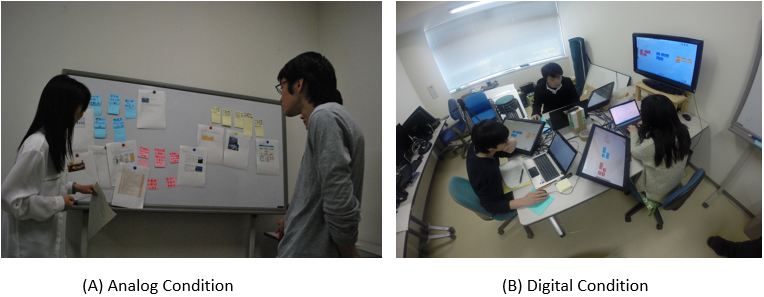
\includegraphics[width=1.0\columnwidth]{condition}
\caption{(A) Analog Condition: using sticky note and white board (B) Digital Condition using DADS with auxiliary multi-touch monitors.}
\label{fig:figure1}
\end{figure}


\section{Instruments and Metrics}

We operationalize usability in three ways: a usability survey administered to participants, a more general System Usability Score, and several behavioral performance metrics. Our analyses test which of the two methods (Digital or Analog) is more preferred by users, and whether DADS supports users in exchanging and organizing their points. We created a detailed survey about specific features and capabilities of the digital and analog conditions, and we also used the Standard Usability Survey to measure the digital system's usability and learnability. We collected data on both user performance and users' self-reported experience, and our analyses highlight the relationships between performance and experience. Correlations between survey items and performance metrics are presented to explore some interesting relationships within the system.

\subsubsection{Survey and Performance Analyses}

We designed a post-experimental questionnaire with 12 1-5 Likert scale questions addressing how easy or hard it was to perform certain tasks using either the Digital or the Analog method. Low scores indicate less reported usability. Questions are listed below with the short item code that we use in graphs and tables throughout this paper. Our specific questions were:

\begin{enumerate}
  \setlength{\itemsep}{1pt}
  \setlength{\parskip}{0pt}
  \setlength{\parsep}{0pt}
  \item How easy was it to create points using this system? (Create)
  \item How easy was it to edit points using this system? (Edit)
  \item How easy was it to attach sources to your points using this system? (Attach)
  \item How easy was it to show resources and support for your points in this system? (Show)
  \item How easy was it to explain your points to others? (Explain)
  \item How easy was it to read other users' points in this system? (Navigate)
  \item How well did you understand other people's points? (Understand)
  %\item How easy was it to read comments on others' points in this system? (Read)
  %\item How easy was it to write comments on others' points in this system? (Write)
  %\item How easy was it to reply to comments in this system? (Reply)
  \item How flexible was it to create an Affinity Diagram in this system? (Flex)
  \item How easy was it for you to cooperate with other group members to achieve the task in this system? (Teamwork)
  \item How comfortable did you feel during the experiment? (Comfort)
  \item How useful do you think this method is compared to the other method you experienced? (Useful)
  \item How satisfied are you with the final Affinity Diagram that you made using this method? (Satisfy)
\end{enumerate}

We measured several aspects of individual users' behavior in order to get a clearer picture of what users did in each of the conditions: number of attachments made, number of comments made, number of times a card was moved, grouped, or linked, and the amount of time groups took  create the final affinity diagram. We also calculated the number of moves per minute for each user. Groups' behavior was recorded automatically in the digital environment. In the analog condition we used a GoPro HERO3+ digital video camera mounted on a jib in order to provide visual access to all users' movements. Video from the analog condition was hand coded by the first author. 

Because all participants experienced both conditions in a randomized order, we used within-subject t-tests to analyze the users' responses and determine whether the two experimental conditions were different from each other. This test is appropriate for our analysis because each participant generates data in both experiments; in essence, we are sampling each participant twice for each measure of the questionnaire and performance metrics. 


%The analysis is based on the differences between the values of each pair - that is, one subtracted from the other. In the formula for within-subjects t-test below, this difference is notated as d.
%\begin{align*}
	%{t} = \frac{\sum d}{ \sqrt{\frac{n(\Sigma d^2) - (\Sigma d)^2}{n-1}}}
%\end{align*}

%We chose p = 0.05 as our threshold for significance for the within-subjects t-tests, reflecting a value of $\alpha$ = 0.05. This value is commonly used in experimental psychology and human factors research, since these fields deal with hypotheses that do not require high levels of certainty in order for significant claims to prove true \cite{bross1971critical}. 

\section{Observation Results}

\begin{table*}[ht]
\centering
\caption {Full Experiment Self reporting Usability Survey result }
\begin{tabular}{lccccccccc}
  \hline
 &  Mean & SD & SE & 95\%LCI & 95\%UCI  & T-Value  & P-Value \\ 
  \hline
Create Points AN  & 3.83 & 1.01 & 0.21 & 3.41 & 4.26  & 1.77  & \color{red}0.09 \\ 
  Create Points DI  & 4.33 & 0.87 & 0.18 & 3.97 & 4.70  &   &  \\ 
    \hline
  Edit Points AN  & 3.12 & 0.95 & 0.19 & 2.73 & 3.52  & 5.88  & 0.00 \\ 
  Edit Points DI  & 4.58 & 0.65 & 0.13 & 4.31 & 4.86  &  &  \\ 
    \hline
  Attach Source AN  & 2.25 & 0.90 & 0.18 & 1.87 & 2.63  & 10.4  & 0.00 \\ 
  Attach Source DI & 4.67 & 0.56 & 0.12 & 4.43 & 4.91  &   &  \\ 
    \hline
  Show Points AN & 2.71 & 1.12 & 0.23 & 2.23 & 3.18  & 6.26  & 0.00 \\ 
  Show Points DI  & 4.54 & 0.72 & 0.15 & 4.24 & 4.85  &   &  \\ 
    \hline
  Explain Points AN  & 3.12 & 0.74 & 0.15 & 2.81 & 3.44  & 2.93  & 0.01 \\ 
  Explain Points DI & 3.71 & 0.69 & 0.14 & 3.42 & 4.00  &   &  \\ 
    \hline
  Navigate Points AN  & 2.96 & 1.08 & 0.22 & 2.50 & 3.42  & 4.46 & 0.00 \\ 
  Navigate Points DI  & 4.29 & 0.86 & 0.18 & 3.93 & 4.65  &  &  \\ 
    \hline
  Understand Points AN  & 3.08 & 0.78 & 0.16 & 2.76 & 3.41  & 3.97  & 0.00 \\ 
  Understand Points DI  & 3.88 & 0.74 & 0.15 & 3.56 & 4.19 &   &  \\ 
    \hline
  %Read Comments AN  & 3.25 & 1.15 & 0.24 & 2.76 & 3.74  & 3.87  & 0.00 \\ 
  %Read Comments  DI  & 4.38 & 0.82 & 0.17 & 4.03 & 4.72  &   &  \\ 
   %%Write Comments AN  & 3.04 & 0.91 & 0.19 & 2.66 & 3.43  & 8.28  & 0.00 \\ 
  %Write Comments  DI  & 4.67 & 0.56 & 0.12 & 4.43 & 4.91  &   &  \\ 
   % \hline
  %Reply Comments AN  & 3.08 & 0.83 & 0.17 & 2.73 & 3.43  & 6.95 & 0.00 \\ 
  %Reply Comments  DI  & 4.46 & 0.66 & 0.13 & 4.18 & 4.74  &   &  \\ 
   % \hline
  Flex  Affinity Diagram AN  & 3.25 & 0.90 & 0.18 & 2.87 & 3.63   & 2.39 & 0.03 \\ 
  Flex  Affinity Diagram DI  & 3.88 & 0.80 & 0.16 & 3.54 & 4.21   & &  \\ 
    \hline
  Teamwork AN  & 3.58 & 0.93 & 0.19 & 3.19 & 3.98  & 0.66  & \color{red}0.52 \\ 
  Teamwork DI  & 3.75 & 0.85 & 0.17 & 3.39 & 4.11  &   &  \\ 
    \hline
  Comfort AN  & 3.46 & 0.72 & 0.15 & 3.15 & 3.76  & 2.11 & 0.04 \\ 
  Comfort DI & 3.92 & 0.93 & 0.19 & 3.52 & 4.31  &   &  \\ 
    \hline
  Usefulness AN  & 3.25 & 0.79 & 0.16 & 2.91 & 3.59  & 6.06  & 0.00 \\ 
  Usefulness DI  & 4.46 & 0.66 & 0.13 & 4.18 & 4.74  &   &  \\ 
    \hline
  Satisfaction AN & 3.42 & 0.72 & 0.15 & 3.11 & 3.72& 6.26 & 0.00 \\ 
  Satisfaction DI  & 4.33 & 0.64 & 0.13 & 4.06 & 4.60  &  &  \\ 
   \hline
\end{tabular}
\end{table*}
We divide the results into 3 areas: 1. Survey measures of usability and user experience, 2. Performance measures of efficient system actions, 3. Correlations between usability and performance. In the first section, we discuss the results of the survey, focusing on 1) Content Creation and Presentation, 2) Navigating, Understanding and Affinity Diagram, and finally 3) Affective Measures in the results. We then check the System Usability Scale for a different perspective on DADS' usability, and to show that the system is scientifically usable based on multiple measurements. In the third section we discuss users' performance based on the performance metrics. Finally, we present a correlation analysis of measures from the survey and user performance to check the strength of our initial hypotheses.
 
\subsubsection{Content Creation and Presentation}

\begin{figure}[!h]
\centering
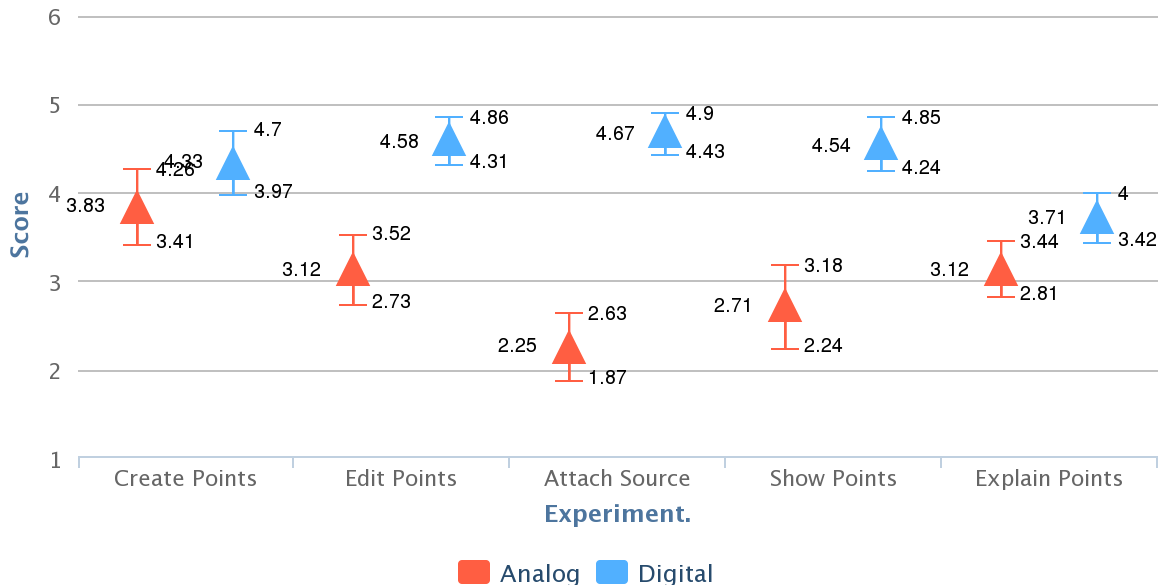
\includegraphics[width=1.0\columnwidth]{Basics}
\caption{Analog and Digital t.test result for creation, editing and understanding}
\label{fig:figure1}
\end{figure}
An analysis of participants' answers to the usability survey questions is shown in the figures below. Within subjects t-tests were used to determine the relative strengths and weaknesses of the two methods (Analog and Digital), as perceived by participants.

Participants reported that it is easier to conduct the tasks involved in creating an affinity diagram using the Digital method compared to the Analog method. The ease of creating, editing, and attaching sources to points was deliberately engineered into our system, as reflected by responses to the usability survey.  Participants found creating points in Digital (M= 4.33, SD = 0.87) to be the same as creating points in Analog (M=3.83, SD = 1.01 p \textless 0.09), however we cannot reject the null hypothesis due high p value therefore we cannot conclude that the Digital system made point creation easier. Editing in digital environment is  significantly easier (M = 4.58, SD = 0.65) than the same process in the Analog condition (M = 3.12, SD = 0.90 p \textless 0.01). This means that users found digital texts easier to edit by deleting and re-typing information, compared to handwritten notes. The Attachment function of DADS proved highly usable, since users rated Attaching sources significantly easier for Digital (M=4.67, SD =0.56) compared to Analog ( M=2.25,SD=0.90, p\textless 0.01). This shows that users found our digital attachment system simpler to use than printing out paper sources to attach to their points. Users report that showing resources to others is easier in the Digital environment (M=4.54, SD=0.72) compared to Analog (M=2.71, SD=1.12, p \textless 0.01). This shows that the presentation tools in our system, such as card expansion and pointer highlighting, both contributed to better usability compared to the Analog method of pasting  the printed sources on the whiteboard. Users also report that it is easier to explain their points in the Digital environment (M=3.71, SD=0.69) compared to Analog (M=3.12, SD=0.74, p \textless 0.05).The design of the digital system made sharing, presenting, and explaining points easier using the digital sources and presentation tools. Participants' rating show us that the separate private and common interfaces improve their ability to edit, support, show and explain points using material they created. These relationships are further explored in the correlation analyses. 
%\subsubsection{Organizing Comments}



%We measured three commenting tasks: 1) Ease of reading comments 2) Ease of writing comments and 3) Ease of replying to comments. While all comment notes are shown in analog, in the digital version the comments are hidden until users choose to read them. The data shows a significant difference between ease of reading in Analog ( M=3.25, SD= 1.15) compared to Digital (M=4.38, SD= 0.88, p \textless 0.01). This shows that participants found it easier to process other participants' comments in the digital interface compared to handwritten notes in analog. Subjects also reported that it is easier to write comments in the Digital system (M=4.67, SD=0.56) compared to writing manually (M=3.04, SD=0.91, p \textless 0.01). This is evidence that creating digital comments felt easier to users than writing a new comment on a card and attaching it to the original point card in the analog method. Users could also reply to comments as they noticed and read them in both experimental conditions. Users rate the Digital format higher for replying to comments (M=4.46, SD= 0.66) than Analog  (M=3.08, SD= 0.83, p \textless 0.01) suggesting that the digital interface made replies easier. Overall, users perceived the digital comment system to be easier to use than the analog comment system.

\subsubsection{Navigating, Understanding and Flexibility}

\begin{figure}[!h]
\centering
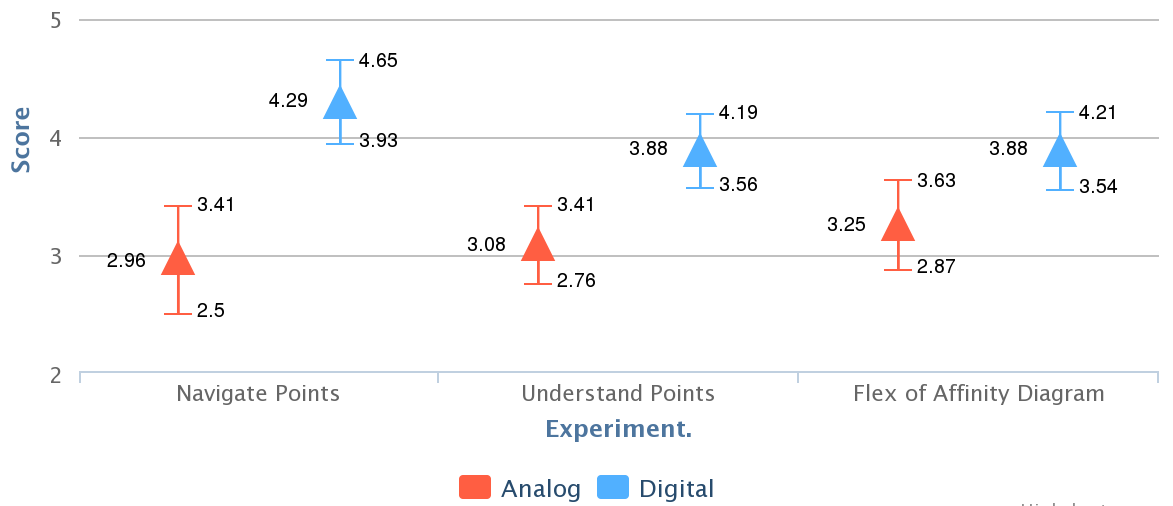
\includegraphics[width=1.0\columnwidth]{nav}
\caption{(A) Analog and Digital T-test result for navigating, understanding and flexibility}
\label{fig:figure1}
\end{figure}

DADS design is intended to improve the ability to navigate between others users points in order to increase readability of the whole discussion contents.  Based on the survey results, users navigated more easily in the Digital environment (M=4.29, SD=0.86) compared to Analog (M=2.96, SD=1.08, p \textless 0.01). This indicates that the digital interface made it easier for users to find and read others' points during the experiment.  In addition, the usability survey asked users how easy it was to understand the discussion content in each condition. Users reported that it is easier to understand the discussion points in digital format (M=3.88, SD=0.80), compared to analog format (M=3.08, SD=0.78, p \textless 0.01) suggesting that users found digitally-presented information easier to understand using the distributed interface than printed or handwritten information presented on a single white board. Regarding the final experiment task, users were asked how easy it was to create the affinity diagram collaboratively, which is a measure of system flexibility. Users rate the digital system as more flexible (M = 3.88 , SD=0.80) than the analog system (M = 3.25, SD=0.90, p \textless 0.05). This result shows that users felt the digital system gave them better flexibility to organize cards to form an affinity diagram than they had in the whiteboard-based analog condition. 

\subsubsection{Affective Metrics}
\begin{figure}[!h]
\centering
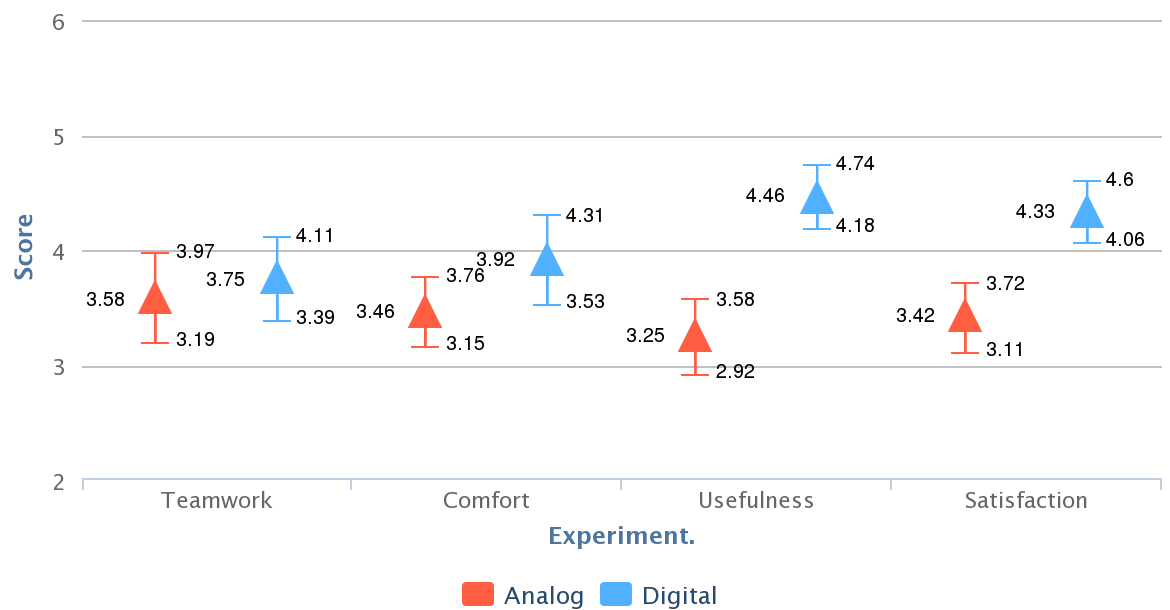
\includegraphics[width=1.0\columnwidth]{affective}
\caption{Analog and Digital t-test result for affective measures}
\label{fig:figure1}
\end{figure}

We also asked users several questions that reflected their general feelings about the system. Users' feelings about teamwork, comfort, usefulness, and satisfaction are subjective, but they are still important factors in making usable systems. 

The usability survey asked users to report how easy it was to collaborate in each system, which is a measure of how well the system promotes teamwork. Upon analyzing, the results showed no statistical difference between the level of teamwork in both Digital (M = 3.75, SD = 0.83) and Analog( M=3.58, SD=1.06, p = 0.52). This indicates that the two process are statistically the same in producing similar level of teamwork collaboration for users. We also asked users how comfortable they were using each system, and participants reported that they felt more comfortable in the Digital system (M = 3.92,SD = 0.93) than the Analog system (M = 3.46, SD = 0.72, p \textless 0.05). This means that users found the distributed digital interfaces more comfortable than the analog process of posting and presenting items using a whiteboard. Users were also asked about the level of usefulness  they thought for  each process, based on the survey, users felt that the digital system was more useful than the analog system (Digital M = 4.46 SD = 0.64, Analog M = 3.27 SD = 0.96, p \textless 0.01) indicating that the functions in digital system is more useful than the analog process. We asked users how satisfied they were in each condition with the collaborative affinity diagram that they made. Users reported higher satisfaction with the outcome of the affinity diagram from the Digital process (M = 4.20, SD = 0.68) compared with the Analog process (M = 3.42, SD = 0.72, p\textless 0.01). The digital system helped users collaborate on a more satisfying result than they produced during the analog condition.

\begin{table}[!htbp] \centering 
  \caption{Performance Metrics Results} 
  \label{} 
\begin{tabular}{@{\extracolsep{-3pt}}llllll} 
\\[-1.8ex]\hline 
\hline \\[-1.8ex] 
Metrics & \multicolumn{1}{c}{AN(SD)} & \multicolumn{1}{c}{DI(SD)} & \multicolumn{1}{c}{P Value}  \\ 
\hline \\[-1.8ex] 
No. Source   & 1.75(1.19)  &    5.50(3.49)    &  \textless0.01    \\
%No.  Comments  & 6.79(1.98)  &    13.25(5.52)    &  \textless0.01    \\
Time Complete AD (min) &    7.11(2.11)   &      15.07(11.10)      &   \textless0.01    \\ 
No.  Card-movement  &    8.04(4.31)& 18.63(14.54)   &  \textless0.01    \\
\hline \\[-1.8ex] 
\normalsize 
\end{tabular} 
\end{table} 


We coded participants' behaviors in both the Analog and Digital conditions, counting the number of sources attached and the number of comments generated. In addition, we also track the number of times users  move the cards during affinity diagram creation and also time the time for the group to complete the affinity diagram sessions. 

 %of times cards were moved and re-grouped, as well as the number of supporting attachments users made to their points. Self-reports from our usability survey are supported by data from users' behavior. 

In the usability survey, users reported that it is easier to attach sources in the digital platform compared to analog methods. This is supported by the difference in the number of sources attached: analog users attached 1.75 source per discussion per person, compared to digital users who attached 5.5 sources per discussion.  This result confirms that the digital attachment feature is more efficient than the method of posting printed sources in the analog condition.
% Ease of commenting was also reported higher for digital users in our survey, which is supported by the number of comments users create during the discussions: each analog user posted on average 6.79 comments per discussion, compared to the digital format where they posted 13.25 comments per discussion. This result shows that users could post comments more efficiently in the digital system compared to the analog pen-and-paper method. 

%Participants felt that it was easier to attach sources in the digital system than in the analog system. This is supported by a greater number of attachments associated with each idea in the digital system (M = 5.50, SD=3.49) than in the analog system (M = 1.75, SD=1.19), p \textless 0.01). This suggests that digital users found the attachment system more usable, thus they used it more. We explore this relationship more in our correlation analysis in order to verify these results.

In the affinity diagram creation phase, participants discussed groups and links that should be created between points, and moved cards to match their discussion. According to the data we collected, these discussions were longer for the digital condition, at a mean of  (M= 15.07 min, SD = 11.10), compared to (M = 7.11 min, SD = 2.11) in the Analog condition. During this time, they moved and grouped cards to create the resulting affinity diagram(AD). The digital system recorded these movements automatically, and we used video to count the number of moves made in the analog condition. We observed that users carried out (M= 18.63, SD = 13.63) card movements per person per discussion in the Digital condition compared to (M=8.04, SD = 1.98) card movements in the Analog condition per person per discussion. This means that users were more active in the Digital creation phase compared to the Analog creation phase. However, it is important to note that Analog and Digital users created the affinity diagram at approximately the same speed. This means that across both conditions, there is no difference between the frequency of move between analog and digital suggesting that users are consistent in pacing their discussion. As reported earlier, Digital users were more satisfied with the result of the affinity diagram. The connection between number of moves and satisfaction will be explored further in our correlation analysis.
\subsection{Correlation Analysis}
Correlations can tell us whether changes in one measure are related to changes in another measure. Several of our hypotheses propose relationships between different results. In order to test these hypotheses, we computed correlation coefficients for select items from the questionnaire and performance metrics in order to explore the relationships between these factors. In order to be conservative, we chose a method that does not assume linearity or consistent variance throughout the data, Spearman's rank correlation ($\rho$)\cite{Myers2003}. Spearman's rank correlation is preferred over Pearson's r in cases where consistent variance in the data cannot be assumed. We chose this analysis method because initial exploration of the data showed some non-linearity. Spearman's $r_{s}$ is calculated as follows:

\begin{align*} % requires amsmath; align* for no eq. number
   { \rho } = { \Sigma_i ( x_i - \bar{x})(y_i - \bar{y}) \over \sqrt{\Sigma_i ( x_i - \bar{x})^2(y_i - \bar{y})^2}} \\
\end{align*}

%Statistical significance for Spearman's $r_{s}$ , as for all correlation tests, is determined by comparing the current test to a 'null hypothesis' that there is no relationship between x and y. P-values of 0.05 or lower will indicate that a correlation is statistically significant. Spearman's $r_{s}$ indicates the strength of the relationship between x and y; if this relationship is shown to be significant, then there is less than 5\% likelihood that the strength of this relationship is due to chance.

\begin{figure*}
\centering
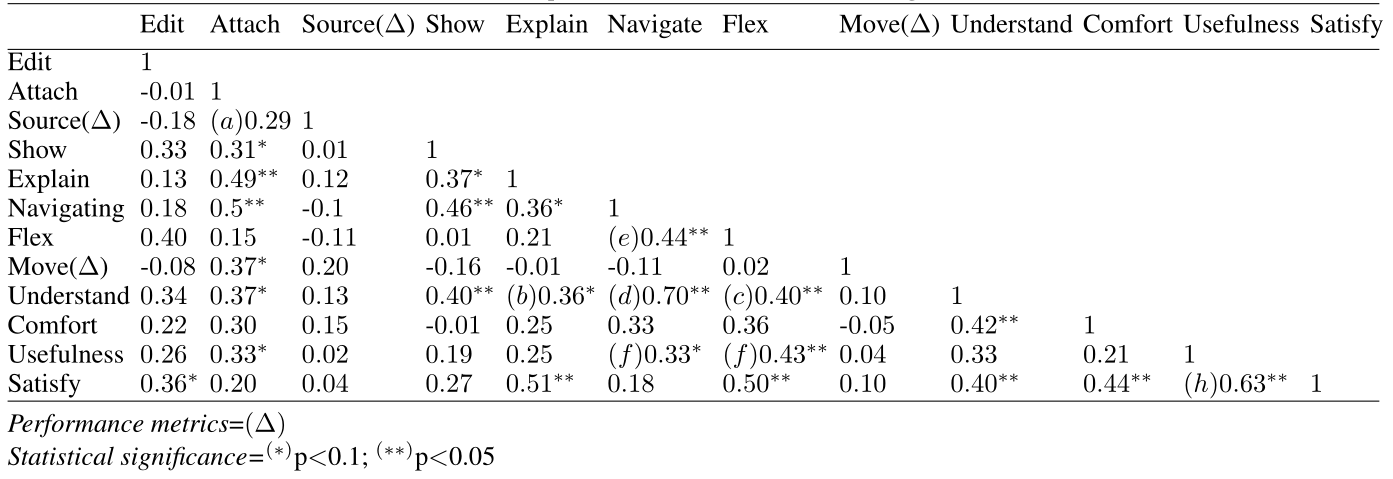
\includegraphics[width=1.6\columnwidth]{spearan}
\caption{ ANALOG Table for Spearman Rho Correlation matrix }
\label{fig:figure1}
\end{figure*}
\begin{figure*}
\centering
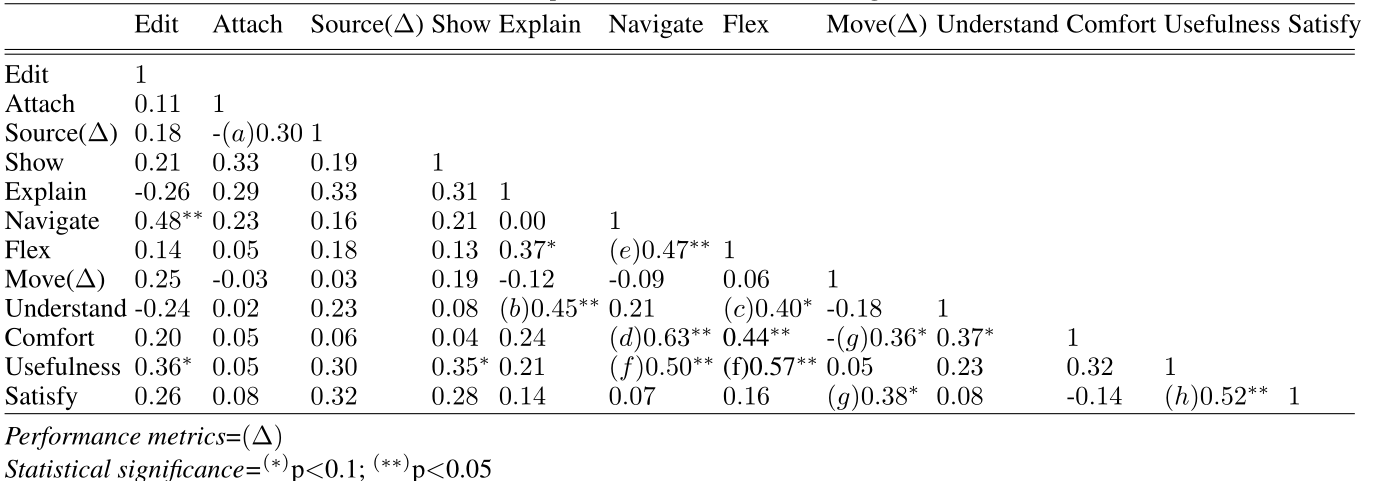
\includegraphics[width=1.6\columnwidth]{speardi}
\caption{ DIGITAL Table for Spearman Rho Correlation matrix }
\label{fig:figure1}
\end{figure*}

While correlations cannot show us a direction of causation, they can show us significant relationships in our data that support our hypotheses. We believe that in group discussion, usability of a system will cause more efficient thinking, greater understanding, and greater satisfaction among participants. These factors will be reflected in the productive actions of users. Our analysis focuses on the correlations that are not only the most significant, but also the most relevant to our hypotheses. We present correlations only between items that showed a significant difference between Analog and Digital conditions in the t-test analysis; this excludes Create Points and Teamwork which show no significant difference between the conditions. 

%Based on our analysis, we discovered that subjects' performance ratings are more stable in Analog compared to Digital. In all of the correlations we measured, there are 13 relationships that are significantly correlated in the Analog condition compared to only 8 in the Digital condition. We believe this is due to familiarity issues with the system; most participants are familiar with analog methods, and they perform and respond in a more similar manner compared to a newly developed system that relies on each participant's level of experience with new technology. 

The analyses we present focus on providing further support for our hypotheses: a) Ease of attachment helps to increase the number of sources used;  b) Number of sources improves explanation and understanding; c) Flexibility also improves understanding; d) Ease of navigation improves understanding; e) Flexibility is related to higher numbers of moves and greater satisfaction with the system. We address each hypothesis in turn below, as well as three additional correlations (f, g, and h) addressing the more subjective questions in our usability questionnaire: usefulness, satisfaction, and comfort.

a) \textbf{Ease of attachment and number of attachment} Our correlation analysis does not provide any evidence that the ease with which the affinity diagram was created had any relation to the number of sources attached. Despite the results of the within-subjects t-test analysis in which users reported that the digital environment made attachments easier, some users did not utilize the attachment function during the experiment, although all users tested this function during the training phase. The perceived usability of the attachment system seemed to have no effect on whether or not the attachment function was used. This may be related to the depth or specific content of users' points, which is outside the scope of this analysis.

b) \textbf{Number of sources, explanation and  understanding} The number of sources used is not correlated with ease of explanation or ease of understanding in either condition. However, ease of explanation and understanding are correlated significantly for the Digital condition ($r_{s}$ = 0.45, p=\textless 0.05). The evidence for this relationship is present, but less clear in Analog ($r_{s}$ = 0.36, p=\textless 0.1). Rather than the volume of sources, users' ease of explanation could play a larger role in their ability to understand other parts of the discussion. 

c) \textbf{Flexibility and understanding} The level of flexibility in creating the affinity diagram is positively correlated with understanding in both conditions. For both Analog and Digital users, this coefficient is ($r_{s}$ = 0.40, p=\textless 0.05). Since we have shown in b) that the number of sources is not correlated with understanding, the data suggests that understanding is more closely related to flexibility than to number of sources. Users who understand all the points better may find it easier to collaborate on an affinity diagram.  

d) \textbf{Navigation, understanding and comfort} Ease of navigation is correlated with understanding in the Analog condition ($r_{s}$ = 0.70, p=\textless 0.05), which supports our hypothesis. However, Digital users' ease of navigation is not correlated with understanding, but with comfort ($r_{s}$ = 0.63, p=\textless 0.05). This suggests that instead of experiencing understanding as related to ease of navigation, digital users may associate understanding with another metric such as explanation, and associate navigation with comfort. As shown in (b), explanation is reported to be correlated to understanding for digital users.  This difference correlation between the two methods should be explored in future research on the role of navigation in usability.

e) \textbf{Navigation and flexibility} The correlation results confirmed that ease of navigation between discussion points and flexibility are correlated in both Analog (($r_{s}$ = 0.44, p=\textless 0.05) and Digital conditions ($r_{s}$ = 0.47, p=\textless 0.05). Flexibility reports the user's experience of how easily they can create an affinity diagram, so this correlation indicates that users who find it easy to navigate  between points  also find it easier to create the collaborative affinity diagram. Flexibility involves moving between different areas, just as navigation does, so users may perceive these two metrics to be similar.

f) \textbf{Navigation, flexibility and usefulness} Ease of navigation is correlated with usefulness for Digital users ($r_{s}$ = 0.49, p=\textless 0.05), while for Analog users the correlation is still positive, but not as strong ($r_{s}$ = 0.325, p=\textless 0.1). However, both conditions showed a relationship between the flexibility of organizing the affinity diagram and perceived usefulness. For Digital users, flexibility and usefulness correlated highly at ($r_{s}$ = 0.57, p=\textless 0.05) and Analog at ($r_{s}$ = 0.40, p=\textless 0.05). This helps us define flexibility of creating affinity diagram as one of the key elements of terms of perception of usefulness.

g) \textbf{Movement, comfort and satisfaction} We were not able to establish a correlation between flexibility and the number of moves in either condition. However, we found interesting potential evidence in the Digital condition where the number of moves is negatively correlated with the level of comfort($r_{s}$ = -0.36, p=\textless 0.1) but positively correlated with the level of satisfaction ($r_{s}$ = 0.38, p=\textless 0.1). This could mean that more movements result in less comfort, but give users more satisfying results. However, Digital user performance varied more than Analog, so these data should still be considered preliminary, prompting further exploration of this new hypothesis.

h) \textbf{Usefulness and satisfaction} Our last correlation shows that Level of Usefulness and Level of Satisfaction are highly correlated for both Analog (($r_{s}$ = 0.63, p=\textless 0.05) and Digital users ($r_{s}$ = 0.52, p=\textless 0.05). This indicates that perceptions of usefulness and satisfaction are closely linked, and that improving the perception usefulness of a system can also improve user satisfaction.
\section{Conclusions}
Overall, exchanging and organizing ideas using the Distributed Affinity Diagram System (DADS) is better received by users in terms of usability, compared to analog methods. The performance metrics showed that users are more productive based on the number of sources and moves made in the digital system.This paper clarifies the usability and efficiency of the design of DADS, and the correlation analysis suggests new hypotheses that can inspire further research in the field of e-Collaboration. Below we present the main insights from this study, and what this work means for future groupware researchers and system designers.

In some ways, DADS met our expectations by making user interactions with the system usable and efficient. Returning to the initial four hypotheses, we can see how the study's results answer the questions proposed: 1) DADS increased the efficiency of content editing and navigation as shown by higher reported ease of editing and ease of navigation in the digital platform. 2) DADS improved the capacity for supportive information sources, shown by the greater number of attachments and ease of attachment in digital. 3) This system made presentation easier, shown by the higher rated ease of explanation in digital. 4) This system increased users' flexibility in collaborating on an affinity diagram, which is evident in the higher rated flexibility of the digital system. These improvements in usability and efficiency are the result of software quality and system design. 

Several other interesting results are worth mentioning: 
\begin{enumerate}
%	\item There was no significant difference between the two methods in terms of how easy it is to create points. This can be attributed to users' openness to digital systems, and suggest that digital input can be at least as efficient as digitizing handwritten notes.
	\item Teamwork is not increased by the distributed digital system. Users did not report different levels of teamwork in the digital platform compared to the analog. The results suggest that doing work on separate screens might be an issue for some users, but not others. We think this discovery is worth further research. 
	\item The number of attachments does not correlate with users' level of understanding. Despite our hypothesis, the results show that the number of attachment available is less important than the ease of presentation, for increasing understanding. This result leads us to propose a theory that clear presentation, not more information, is the best way to increase users' understanding. 
	\item In the digital platform, increased movements during affinity diagram creation is negatively correlated with level of comfort. This means there is a general tendency that the more moves a user makes, the more uncomfortable they are. However, the results of the correlation analysis link the number of movements to the level of satisfaction, which means that even though it is less comfortable to engage in more movement, the users felt more satisfied with the final results. These results suggest a potential pattern, but they should not be seen as conclusive.
\end{enumerate}

The results of this study suggest that future research should focus on two things: 1) designing a user interface that allows users to organize users' points flexibly, and 2) including presentation features that support better explanation and understanding. These two functions are important to consider when building future systems. In order to build highly usable systems, future designers should also focus on the quality of the software, minimizing response time and working to correct all software bugs so that user experience is optimized. The results also suggest that scholars do further research on the relationship between distributed screens and teamwork. 

%Despite the high usability, we acknowledge the challenges of teamwork using distributed screen, In our  results, we do not see a difference between the two analog and digital, thus the research of distributed interactive screen. 

Despite evidence that our system increases usability, we acknowledge the challenges of teamwork using a distributed-screen system. Based on this experiment, we were able to determine that the digital system's individual screens might prevent higher levels of perceived teamwork. In our results, we do not detect a difference between analog and digital in terms of teamwork. Almost all the other indicators that we measured show that DADS is more usable than the analog method. Thus, the result from teamwork does not lessen DADS' usefulness as a system for collaborative idea exchange. Future research can explore which parts of distributed interaction systems affect teamwork most.

Digital collaboration systems have already addressed some of the efficiency and usability problems that analog tools have. DADS is an integrated system for digital collaboration that builds on previous work to improve a common way that teams share ideas, making communication more efficient during affinity diagram creation. Our research into the usability of this system provides insight into the way distributed workspaces can improve collaborative discussion by making it easier to share ideas, easier to present and support these ideas with accessible material, and increase satisfaction with the outcome of the discussion. The insights in our detailed usability study can provide new and fruitful directions for researchers in computer-supported collaborative work (CSCW) to explore.

\section{Acknowledgments}

We would like to extend our gratitude to  the University for providing laboratory facilities, and the  Ministry of Education, Culture, Sports, Science and Technology for government funding and scholarship.


\bibliographystyle{acm-sigchi}
\bibliography{sample}
\end{document}
